%Version 2.1 April 2023
% See section 11 of the User Manual for version history
%
%%%%%%%%%%%%%%%%%%%%%%%%%%%%%%%%%%%%%%%%%%%%%%%%%%%%%%%%%%%%%%%%%%%%%%
%%                                                                 %%
%% Please do not use \input{...} to include other tex files.       %%
%% Submit your LaTeX manuscript as one .tex document.              %%
%%                                                                 %%
%% All additional figures and files should be attached             %%
%% separately and not embedded in the \TeX\ document itself.       %%
%%                                                                 %%
%%%%%%%%%%%%%%%%%%%%%%%%%%%%%%%%%%%%%%%%%%%%%%%%%%%%%%%%%%%%%%%%%%%%%

\documentclass[sn-apa,pdflatex]{sn-jnl}

%%%% Standard Packages
%%<additional latex packages if required can be included here>

\usepackage{graphicx}%
\usepackage{multirow}%
\usepackage{amsmath,amssymb,amsfonts}%
\usepackage{amsthm}%
\usepackage{mathrsfs}%
\usepackage[title]{appendix}%
\usepackage{xcolor}%
\usepackage{textcomp}%
\usepackage{manyfoot}%
\usepackage{booktabs}%
\usepackage{algorithm}%
\usepackage{algorithmicx}%
\usepackage{algpseudocode}%
\usepackage{listings}%
%%%%

%%%%%=============================================================================%%%%
%%%%  Remarks: This template is provided to aid authors with the preparation
%%%%  of original research articles intended for submission to journals published
%%%%  by Springer Nature. The guidance has been prepared in partnership with
%%%%  production teams to conform to Springer Nature technical requirements.
%%%%  Editorial and presentation requirements differ among journal portfolios and
%%%%  research disciplines. You may find sections in this template are irrelevant
%%%%  to your work and are empowered to omit any such section if allowed by the
%%%%  journal you intend to submit to. The submission guidelines and policies
%%%%  of the journal take precedence. A detailed User Manual is available in the
%%%%  template package for technical guidance.
%%%%%=============================================================================%%%%

\geometry{
  left=2cm,
  right=2cm,
  top=2cm,
  bottom=2cm
} % Modify the margins of the template
\setlength{\parskip}{6pt} % Increase space between paragraphs
\usepackage{fvextra}
\DefineVerbatimEnvironment{Highlighting}{Verbatim}{breaklines,commandchars=\\\{\}}

\usepackage{booktabs}
\usepackage{longtable}
\usepackage{array}
\usepackage{multirow}
\usepackage{wrapfig}
\usepackage{float}
\usepackage{colortbl}
\usepackage{pdflscape}
\usepackage{tabu}
\usepackage{threeparttable}
\usepackage{threeparttablex}
\usepackage[normalem]{ulem}
\usepackage{makecell}
\usepackage{xcolor}


\raggedbottom



% Pandoc syntax highlighting
\usepackage{color}
\usepackage{fancyvrb}
\newcommand{\VerbBar}{|}
\newcommand{\VERB}{\Verb[commandchars=\\\{\}]}
\DefineVerbatimEnvironment{Highlighting}{Verbatim}{commandchars=\\\{\}}
% Add ',fontsize=\small' for more characters per line
\usepackage{framed}
\definecolor{shadecolor}{RGB}{248,248,248}
\newenvironment{Shaded}{\begin{snugshade}}{\end{snugshade}}
\newcommand{\AlertTok}[1]{\textcolor[rgb]{0.94,0.16,0.16}{#1}}
\newcommand{\AnnotationTok}[1]{\textcolor[rgb]{0.56,0.35,0.01}{\textbf{\textit{#1}}}}
\newcommand{\AttributeTok}[1]{\textcolor[rgb]{0.13,0.29,0.53}{#1}}
\newcommand{\BaseNTok}[1]{\textcolor[rgb]{0.00,0.00,0.81}{#1}}
\newcommand{\BuiltInTok}[1]{#1}
\newcommand{\CharTok}[1]{\textcolor[rgb]{0.31,0.60,0.02}{#1}}
\newcommand{\CommentTok}[1]{\textcolor[rgb]{0.56,0.35,0.01}{\textit{#1}}}
\newcommand{\CommentVarTok}[1]{\textcolor[rgb]{0.56,0.35,0.01}{\textbf{\textit{#1}}}}
\newcommand{\ConstantTok}[1]{\textcolor[rgb]{0.56,0.35,0.01}{#1}}
\newcommand{\ControlFlowTok}[1]{\textcolor[rgb]{0.13,0.29,0.53}{\textbf{#1}}}
\newcommand{\DataTypeTok}[1]{\textcolor[rgb]{0.13,0.29,0.53}{#1}}
\newcommand{\DecValTok}[1]{\textcolor[rgb]{0.00,0.00,0.81}{#1}}
\newcommand{\DocumentationTok}[1]{\textcolor[rgb]{0.56,0.35,0.01}{\textbf{\textit{#1}}}}
\newcommand{\ErrorTok}[1]{\textcolor[rgb]{0.64,0.00,0.00}{\textbf{#1}}}
\newcommand{\ExtensionTok}[1]{#1}
\newcommand{\FloatTok}[1]{\textcolor[rgb]{0.00,0.00,0.81}{#1}}
\newcommand{\FunctionTok}[1]{\textcolor[rgb]{0.13,0.29,0.53}{\textbf{#1}}}
\newcommand{\ImportTok}[1]{#1}
\newcommand{\InformationTok}[1]{\textcolor[rgb]{0.56,0.35,0.01}{\textbf{\textit{#1}}}}
\newcommand{\KeywordTok}[1]{\textcolor[rgb]{0.13,0.29,0.53}{\textbf{#1}}}
\newcommand{\NormalTok}[1]{#1}
\newcommand{\OperatorTok}[1]{\textcolor[rgb]{0.81,0.36,0.00}{\textbf{#1}}}
\newcommand{\OtherTok}[1]{\textcolor[rgb]{0.56,0.35,0.01}{#1}}
\newcommand{\PreprocessorTok}[1]{\textcolor[rgb]{0.56,0.35,0.01}{\textit{#1}}}
\newcommand{\RegionMarkerTok}[1]{#1}
\newcommand{\SpecialCharTok}[1]{\textcolor[rgb]{0.81,0.36,0.00}{\textbf{#1}}}
\newcommand{\SpecialStringTok}[1]{\textcolor[rgb]{0.31,0.60,0.02}{#1}}
\newcommand{\StringTok}[1]{\textcolor[rgb]{0.31,0.60,0.02}{#1}}
\newcommand{\VariableTok}[1]{\textcolor[rgb]{0.00,0.00,0.00}{#1}}
\newcommand{\VerbatimStringTok}[1]{\textcolor[rgb]{0.31,0.60,0.02}{#1}}
\newcommand{\WarningTok}[1]{\textcolor[rgb]{0.56,0.35,0.01}{\textbf{\textit{#1}}}}

% tightlist command for lists without linebreak
\providecommand{\tightlist}{%
  \setlength{\itemsep}{0pt}\setlength{\parskip}{0pt}}





\begin{document}


\title[Atlas ictiogeográfico de la Patagonia]{Atlas ictiogeográfico de
la Patagonia occidental: homologción y consolidación de bases de datos}

%%=============================================================%%
%% Prefix	-> \pfx{Dr}
%% GivenName	-> \fnm{Joergen W.}
%% Particle	-> \spfx{van der} -> surname prefix
%% FamilyName	-> \sur{Ploeg}
%% Suffix	-> \sfx{IV}
%% NatureName	-> \tanm{Poet Laureate} -> Title after name
%% Degrees	-> \dgr{MSc, PhD}
%% \author*[1,2]{\pfx{Dr} \fnm{Joergen W.} \spfx{van der} \sur{Ploeg} \sfx{IV} \tanm{Poet Laureate}
%%                 \dgr{MSc, PhD}}\email{iauthor@gmail.com}
%%=============================================================%%

\author*[1]{\fnm{Cristian} \sur{Correa} }\email{\href{mailto:cristiancorrea@gmail.com}{\nolinkurl{cristiancorrea@gmail.com}}}

\author[1]{\fnm{Maryse} \sur{Boisjoly} }



  \affil[1]{\orgdiv{Instituto de Conservación Biodiversidad y
Territorio}, \orgname{Universidad Austral de
Chile}, \orgaddress{\city{Valdivia}, \country{Chile}}}

\abstract{Por encargo del Programa Austral Patagonia (ProAP) de The Pew
Charitable Trusts, se presenta una recopilación de información detallada
de ocurrencia de peces de agua dulce, estuarinos y diadromos en la
Patagonia occidental (40.8-56.0°S). Aquí se documenta en detalle la
recopilación, análisis, y combinación de 12 conjuntos de datos de
ocurrencias, obtenidos empíricamente (a travéz de prospecciones
ictiológicas), a partir de revisiones de literatura, y de distintas
bases de datos. El resultado es una base de datos geográfica de
ocurrencia de peces en formato compatible con el Darwin Core standard.
Hemos llamado al set de datos resultante Atlas Ictiogeográfico de la
Patagonia Occidental.}

\keywords{peces de agua dulce / freshwater fish, datos de ocurrencia /
occurrence data, biomonitoreo / biomonitoring, GBIF, Darwin
Core, Patagonia occidental / Western Patagonia, Ecology, Conservation
biology}



\maketitle

\newpage
\setcounter{tocdepth}{3}
\renewcommand{\contentsname}{Tabla de Contenidos}
\tableofcontents
\newpage

\textbf{Nota: Esta versión preliminar contiene etiquetas indicando
detalles que necesitan atención por parte del los autores. Las etiquetas
se identifican con el texto {[}HERE{]}.}

\section{Introduction}\label{sec1}

Los ecosistemas dulceacuícolas tienen un alto grado de amenaza a nivel
mundial \citep{Dudgeon2006}. Patagonia occidental no es una excepción, a
pesar de la gran cobertura de áreas protegidas. Desde las vulnerables
cabeceras de los ríos, y tramos inferiores que están excluidos desde las
áreas protegidas, hasta el gran desconocimiento del estado poblacional y
distribución de muchas especies dulceacuícolas \citep{Reid2021}.

En el contexto de un primer esfuerzo regional en avanzar en la
planificación de la conservación dulceacuícola en la Patagonia
occidental, se desarrolló el informe ``Priorización de cuencas para la
conservación en Patagonia'' \citep{Aguilar2022}, donde se identificaron
tres ejes de avance: (1) la consolidación de información de
biodiversidad de tres grupos taxonómicos dulceacuícolas, (2) la
identificación de \textbf{subrogantes} geoespaciales que destaquen
valores de conservación dulceacuícola, y (3) el desarrollo de un
prototipo metodológico para la priorización de múltiples valores de
conservación dulceacuícola a la escala de sub-subcuenca.\\
Una de las principales limitantes en esta primera iteración fue la
carencia de información sobre biodiversidad dulceacuícola, donde resalta
fuertemente el poco conocimiento y la baja densidad de observaciones
comparado con otros esfuerzos similares en otras áreas geográficas
\citep[p.~26]{Aguilar2022}.

Aunque la literatura científica es una fuente importante de información
sobre biodiversidad, también hay mucha información de las especies
dulceacuícolas en la literatura gris, entidades estatales, bases de dato
publicas GBIF y iNaturalist, y, finalmente, en el conocimiento de
las/los expertos/as taxónomos y naturalistas. Mucho conocimiento e
información que queda en las bases de dato de estos especialistas, que
aún no es transcrita a observaciones oficiales, lo cual se relaciona
directamente al escaso financiamiento para el trabajo de especialistas.
Por lo tanto, una de las recomendaciones principales en este informe y
de \citet{Reid2021} fue mejorar la información de biodiversidad
integrando al grupo de trabajo a los/as expertas, que con su
conocimiento especializado en cada grupo taxonómico lograrían mejorar,
consolidar y evaluar las observaciones existentes de biodiversidad. Este
atlas ictiográfico es el resultado de este esfuerzo, y también un
ejemplo a seguir para otros grupos dulceacuícolas.

El presente documento detalla la metodología en la revisión del material
existente, la recopilación, análisis, y combinación de diversos
conjuntos de datos de ocurrencias de peces dulceacuícolas y diádromos
obtenidos empíricamente (a través de prospecciones ictiológicas), a
partir de revisiones de literatura, y de distintas bases de datos. El
resultado es una base de datos geográfica de ocurrencia de peces en
formato compatible con el Darwin Core standard (DwC), un estándar
ampliamente adoptado para la distribución y consolidación de bases de
datos biológicas de ocurrencia de especies por entidades tales como el
Global Biodiversity Information Facility
(\href{https://www.gbif.org/}{GBIF}) o la Superintendencia del Medio
Ambiente, Gobierno de Chile.

\section{Estrategia metodológica}\label{sec2}

La estrategia metodológica usada para combinar los conjuntos de datos se
puede describir a grandes rasgos en cinco partes:

\begin{enumerate}
\def\labelenumi{\arabic{enumi}.}
\item
  Cada set de datos fue visualizado en un mapa y revisado para
  identificar y corregir inconsistencias y errores.
\item
  Se homologaron los campos o atributos disponibles (columnas) en cada
  conjunto de datos con aquellos disponibles en el DwC (ver planilla
  \texttt{Atlas\_Ictiogeografico\_Homologacion.xlsx}). Básicamente, los
  nombres de las columnas de cada conjunto de datos fueron reemplazados
  por los nombres de los mismos atributos del DwC, y en algunos casos se
  combinaron los campos originales para producir uno homologado.
\item
  A cada conjunto de datos se le añadieron atributos (columnas) del DwC
  que son aplicables y propios a cada uno en su totalidad, tal como
  nombre del conjunto de datos (\texttt{datasetName}).
\item
  Los conjuntos de datos se combinaron en una gran base de datos
  geográfica reteniendo el mayor número posible de atributos
  homologados. Esta fue llamada \textbf{Atlas Ictiogeográfico de la
  Patagonia Occidental} y es el principal producto de este análisis.
\item
  Dado que hubo considerable redundancia entre conjuntos de datos, el
  atlas ictiogeográfico fue examinado de diferentes formas para
  identificar ocurrencias duplicadas (e.g., mismo registro reportado en
  dos o más conjuntos de datos). Para esto, se usaron tanto pruebas
  programáticas tal como la identificación de fechas y coordenadas
  repetidas dentro de un rango acotado, como inspección manual de la
  tabla de atributos a una escala geográfica fina (e.g., sub-cuenca).
\end{enumerate}

En los siguientes capítulos se documenta detalladamente (código R y
prosa breve) la adopción del estándar DwC, el proceso de homologación (y
otras manipulaciones) de cada conjunto de datos, y el refinamiento y
consolidación del atlas ictiogeográfico. Al final, se presenta una breve
sección de resultados preliminares examinando el contenido general del
Atlas.

Se trabajó en

\begin{Shaded}
\begin{Highlighting}[]
\NormalTok{R.version}
\end{Highlighting}
\end{Shaded}

\begin{verbatim}
##                _                                
## platform       x86_64-w64-mingw32               
## arch           x86_64                           
## os             mingw32                          
## crt            ucrt                             
## system         x86_64, mingw32                  
## status                                          
## major          4                                
## minor          4.1                              
## year           2024                             
## month          06                               
## day            14                               
## svn rev        86737                            
## language       R                                
## version.string R version 4.4.1 (2024-06-14 ucrt)
## nickname       Race for Your Life
\end{verbatim}

Al final de este documento se presenta la información completa de la
sesión de trabajo en R.

\section{Estándar Darwin Core (DwC)}\label{estuxe1ndar-darwin-core-dwc}

``El \emph{Darwin Core} (DwC) \citep{Wieczorek2012} es un estándar
mantenido por el Grupo de Interés de Mantenimiento de Darwin Core
(Darwin Core Maintenance Interest Group). Incluye un glosario de
términos (en otros contextos podrían llamarse propiedades, elementos,
campos, columnas, atributos o conceptos) destinados a facilitar el
intercambio de información sobre la diversidad biológica al proporcionar
identificadores, etiquetas y definiciones. DwC se basa principalmente en
taxa, su presencia en la naturaleza documentada por observaciones,
especímenes, muestras e información relacionada.'' (traducido de
\url{https://github.com/tdwg/dwc}).

La adopción de un estándar es importante porque fomenta la
interoperabilidad entre distintas plataformas y herramientas para el
estudio y gestión de la biodiversidad a nivel internacional. El DwC es
posiblemente el estándar vigente más ampliamente aceptado
internacionalmente para datos de ocurrencia de especies.

La distribución del estándar se hace a través del portal GitHub del
Darwin Core Maintenance Interest Group
\url{https://github.com/tdwg/dwc}. Allí se encuentran definiciones,
etiquetas, ejemplos, versiones anteriores, entre otros recursos, que a
su vez son reflejados en una guía más fácil de leer
(\href{https://dwc.tdwg.org/terms/}{Darwin Core Quick Reference Guide}).

Una lista de 179 atributos o campos (vigentes y obsoletos) con sus
respectivas definiciones, etc., fue obtenida de
\href{https://github.com/tdwg/dwc/blob/master/vocabulary/term_versions.csv}{GitHub
(versión 2023-04-28)}, y de estos una fracción (\textasciitilde36) de
los atributos vigentes fue considerado con algún grado de prioridad para
los efectos de este proyecto, incluyendo aquellos destacados por la red
GBIF como
\href{https://ipt.gbif.org/manual/en/ipt/latest/darwin-core}{campos
primarios y campos obligatorios}. La lista completa de atributos y la
priorización de esta está disponible en un archivo suplementario
(\texttt{input\_parameters/Atlas\_Ictiogeografico\_Homologacion.xlsx}).
A continuación se reproduce parte de la lista de atributos seleccionados
(Table \ref{tab:Table1}).

Es importante destacar que el campo \texttt{eventDate} en el DwC tolera
diferentes formatos tales como 2025-11-29 (año), 2025-11 (mes), 2025
(año), e incluso intervalos de tiempo 2023-09-05/2023-09-18
\url{https://techdocs.gbif.org/en/data-processing/temporal-interpretation}.

\begin{Shaded}
\begin{Highlighting}[]
\NormalTok{DwC }\OtherTok{\textless{}{-}}\NormalTok{ readxl}\SpecialCharTok{::}\FunctionTok{read\_xlsx}\NormalTok{(}\StringTok{"input\_parameters/Atlas\_Ictiogeografico\_Homologacion.xlsx"}\NormalTok{,}
    \AttributeTok{sheet =} \StringTok{"Matriz de homologacion"}\NormalTok{, }\AttributeTok{skip =} \DecValTok{9}\NormalTok{)}
\end{Highlighting}
\end{Shaded}

Selección de campos que se consideraron prioritarios para este proyecto

\begin{Shaded}
\begin{Highlighting}[]
\NormalTok{DwC.keep }\OtherTok{\textless{}{-}}\NormalTok{ DwC }\SpecialCharTok{\%\textgreater{}\%}
    \FunctionTok{filter}\NormalTok{(}\SpecialCharTok{!}\FunctionTok{is.na}\NormalTok{(}\StringTok{\textasciigrave{}}\AttributeTok{Prioridad campo (MB\_CC)}\StringTok{\textasciigrave{}}\NormalTok{))}

\CommentTok{\# table(DwC.keep$\textasciigrave{}Prioridad campo (MB\_CC)\textasciigrave{})}
\end{Highlighting}
\end{Shaded}

\begin{longtable}[t]{>{\raggedright\arraybackslash}p{15em}>{\raggedright\arraybackslash}p{30em}}
\caption{\label{tab:Table1}Atributos seleccionados del estándar Darwin Core y su definición. Más detalles y ejemplos de cada uno en archivo excel suplementario.}\\
\toprule
Darwin Core Terms (DwC) & definition (DwC)\\
\midrule
license & A legal document giving official permission to do something with the resource.\\
rightsHolder & A person or organization owning or managing rights over the resource.\\
accessRights & Information about who can access the resource or an indication of its security status.\\
bibliographicCitation & A bibliographic reference for the resource as a statement indicating how this record should be cited (attributed) when used.\\
references & A related resource that is referenced, cited, or otherwise pointed to by the described resource.\\
\addlinespace
institutionID & An identifier for the institution having custody of the object(s) or information referred to in the record.\\
collectionID & An identifier for the collection or dataset from which the record was derived.\\
institutionCode & The name (or acronym) in use by the institution having custody of the object(s) or information referred to in the record.\\
collectionCode & The name, acronym, coden, or initialism identifying the collection or data set from which the record was derived.\\
datasetName & The name identifying the data set from which the record was derived.\\
\addlinespace
basisOfRecord & The specific nature of the data record.\\
occurrenceID & An identifier for the Occurrence (as opposed to a particular digital record of the occurrence). In the absence of a persistent global unique identifier, construct one from a combination of identifiers in the record that will most closely make the occurrenceID globally unique.\\
catalogNumber & An identifier (preferably unique) for the record within the data set or collection.\\
recordNumber & An identifier given to the Occurrence at the time it was recorded. Often serves as a link between field notes and an Occurrence record, such as a specimen collector's number.\\
recordedBy & A list (concatenated and separated) of names of people, groups, or organizations responsible for recording the original Occurrence. The primary collector or observer, especially one who applies a personal identifier (recordNumber), should be listed first.\\
\addlinespace
individualCount & The number of individuals present at the time of the Occurrence.\\
organismQuantity & A number or enumeration value for the quantity of organisms.\\
organismQuantityType & The type of quantification system used for the quantity of organisms.\\
lifeStage & The age class or life stage of the Organism(s) at the time the Occurrence was recorded.\\
associatedReferences & A list (concatenated and separated) of identifiers (publication, bibliographic reference, global unique identifier, URI) of literature associated with the Occurrence.\\
\addlinespace
otherCatalogNumbers & A list (concatenated and separated) of previous or alternate fully qualified catalog numbers or other human-used identifiers for the same Occurrence, whether in the current or any other data set or collection.\\
eventDate & The date-time or interval during which an Event occurred. For occurrences, this is the date-time when the event was recorded. Not suitable for a time in a geological context.\\
year & The four-digit year in which the Event occurred, according to the Common Era Calendar.\\
verbatimEventDate & The verbatim original representation of the date and time information for an Event.\\
samplingProtocol & The names of, references to, or descriptions of the methods or protocols used during an Event.\\
\addlinespace
samplingEffort & The amount of effort expended during an Event.\\
waterBody & The name of the water body in which the Location occurs.\\
locality & The specific description of the place.\\
decimalLatitude & The geographic latitude (in decimal degrees, using the spatial reference system given in geodeticDatum) of the geographic center of a Location. Positive values are north of the Equator, negative values are south of it. Legal values lie between -90 and 90, inclusive.\\
decimalLongitude & The geographic longitude (in decimal degrees, using the spatial reference system given in geodeticDatum) of the geographic center of a Location. Positive values are east of the Greenwich Meridian, negative values are west of it. Legal values lie between -180 and 180, inclusive.\\
\addlinespace
coordinateUncertaintyInMeters & The horizontal distance (in meters) from the given decimalLatitude and decimalLongitude describing the smallest circle containing the whole of the Location. Leave the value empty if the uncertainty is unknown, cannot be estimated, or is not applicable (because there are no coordinates). Zero is not a valid value for this term.\\
typeStatus & A list (concatenated and separated) of nomenclatural types (type status, typified scientific name, publication) applied to the subject.\\
scientificName & The full scientific name, with authorship and date information if known. When forming part of an Identification, this should be the name in lowest level taxonomic rank that can be determined. This term should not contain identification qualifications, which should instead be supplied in the IdentificationQualifier term.\\
kingdom & The full scientific name of the kingdom in which the taxon is classified.\\
family & The full scientific name of the family in which the taxon is classified.\\
\addlinespace
genus & The full scientific name of the genus in which the taxon is classified.\\
\bottomrule
\end{longtable}

En el capítulo \emph{Conjuntos de datos analizados} se presenta, uno a
la vez, cada conjunto de datos con una breve descripción y la forma en
que fue homologado para conformar el estándar DwC.

\section{Listado taxonómico de
peces}\label{listado-taxonuxf3mico-de-peces}

Algunas bases de datos globales requirieron ser filtradas para obtener
ocurrencias de peces de interés para este proyecto, y este proceso se
hizo basado en criterios geográficos y taxonomicos. Para el criterio
taxonómico, este se dividió en dos etapas, una \emph{a pripori} y otra
\emph{a posteriori}.

En ambos casos se adoptó la clasificación taxonómica de \emph{GBIF
Backbone Taxonomy}
(\href{https://www.gbif.org/dataset/d7dddbf4-2cf0-4f39-9b2a-bb099caae36c}{\citet{GBIF-Secretariat2023}}).

\begin{itemize}
\tightlist
\item
  Filtrado taxonómico \emph{a priori}: Dentro de lo posible, se
  retuvieron todas las especies de peces (incluso marinas) hasta
  consolidar la base de datos homologada, y solo entonces se filtró para
  retener el conjunto de especies de nuestro interés (i.e., Filtrado
  taxonómico \emph{a posteriori}). Para obtener datos de peces de
  algunos motores de búsqueda masiva (e.g., GBIF), se hizo una lista
  completa (inclusiva) de ordenes de peces, para usarla como criterio de
  búsqueda. Este paso fue necesario porque la clase Actinopterygii ya no
  se considera un grupo taxonómico válido en el \emph{GBIF Backbone
  Taxonomy} porque no es monofilético, lo que significa que no incluye a
  todos los descendientes de un solo ancestro común (Table
  \ref{tab:fish_orders}).
\end{itemize}

\begin{Shaded}
\begin{Highlighting}[]
\NormalTok{res }\OtherTok{\textless{}{-}} \FunctionTok{name\_lookup}\NormalTok{(}\AttributeTok{rank =} \StringTok{"order"}\NormalTok{, }\AttributeTok{higherTaxonKey =} \DecValTok{44}\NormalTok{, }\AttributeTok{isExtinct =}\NormalTok{ F,}
    \AttributeTok{limit =} \DecValTok{200}\NormalTok{)}

\CommentTok{\# res$meta$count \# Number of records available}
\CommentTok{\# gbif\_names(res) \# online result viewer}

\CommentTok{\# Filter fish orders (other taxa display classes in}
\CommentTok{\# \textquotesingle{}parent\textquotesingle{})}
\NormalTok{fish.orders }\OtherTok{\textless{}{-}}\NormalTok{ res}\SpecialCharTok{$}\NormalTok{data }\SpecialCharTok{\%\textgreater{}\%}
    \FunctionTok{filter}\NormalTok{(parent }\SpecialCharTok{==} \StringTok{"Chordata"}\NormalTok{)}
\end{Highlighting}
\end{Shaded}

\begingroup\fontsize{7}{9}\selectfont

\begin{longtable}[t]{>{\raggedright\arraybackslash}p{10em}>{\raggedleft\arraybackslash}p{8em}>{\raggedright\arraybackslash}p{10em}>{\raggedright\arraybackslash}p{15em}}
\caption{\label{tab:fish_orders}Ordenes de peces incluidos en la lista de búsqueda a priori.}\\
\toprule
order & orderKey & taxonomicStatus & habitats\\
\midrule
Acipenseriformes & 1103 & ACCEPTED & FRESHWATER, MARINE\\
Albuliformes & 1104 & ACCEPTED & FRESHWATER, MARINE\\
Amiiformes & 494 & ACCEPTED & FRESHWATER, MARINE\\
Anguilliformes & 495 & ACCEPTED & FRESHWATER, MARINE\\
Ateleopodiformes & 1105 & ACCEPTED & MARINE\\
\addlinespace
Atheriniformes & 496 & ACCEPTED & FRESHWATER, MARINE\\
Aulopiformes & 497 & ACCEPTED & MARINE\\
Batrachoidiformes & 1106 & ACCEPTED & FRESHWATER, MARINE\\
Beloniformes & 498 & ACCEPTED & FRESHWATER, MARINE\\
Beryciformes & 499 & ACCEPTED & MARINE\\
\addlinespace
Cetomimiformes & 1107 & ACCEPTED & MARINE\\
Characiformes & 537 & ACCEPTED & FRESHWATER, MARINE\\
Clupeiformes & 538 & ACCEPTED & FRESHWATER, MARINE\\
Cypriniformes & 1153 & ACCEPTED & FRESHWATER, MARINE\\
Cyprinodontiformes & 547 & ACCEPTED & FRESHWATER, MARINE\\
\addlinespace
Elopiformes & 1162 & ACCEPTED & FRESHWATER, MARINE\\
Esociformes & 548 & ACCEPTED & FRESHWATER\\
Gadiformes & 549 & ACCEPTED & FRESHWATER, MARINE\\
Gasterosteiformes & 550 & ACCEPTED & FRESHWATER, MARINE\\
Gobiesociformes & 1163 & ACCEPTED & FRESHWATER, MARINE\\
\addlinespace
Gymnotiformes & 1165 & ACCEPTED & FRESHWATER\\
Lampriformes & 1166 & ACCEPTED & MARINE\\
Lepisosteiformes & 1167 & ACCEPTED & FRESHWATER, MARINE\\
Lophiiformes & 1305 & ACCEPTED & MARINE\\
Mugiliformes & 1067 & ACCEPTED & FRESHWATER, MARINE\\
\addlinespace
Myctophiformes & 1306 & ACCEPTED & MARINE\\
Notacanthiformes & 1307 & ACCEPTED & MARINE\\
Ophidiiformes & 1308 & ACCEPTED & FRESHWATER, MARINE\\
Osmeriformes & 1068 & ACCEPTED & FRESHWATER, MARINE\\
Osteoglossiformes & 1069 & ACCEPTED & FRESHWATER, MARINE\\
\addlinespace
Perciformes & 587 & ACCEPTED & FRESHWATER, MARINE\\
Percopsiformes & 1310 & ACCEPTED & FRESHWATER\\
Pleuronectiformes & 588 & ACCEPTED & FRESHWATER, MARINE\\
Polymixiiformes & 589 & ACCEPTED & MARINE\\
Polypteriformes & 1311 & ACCEPTED & FRESHWATER\\
\addlinespace
Saccopharyngiformes & 1312 & ACCEPTED & MARINE\\
Salmoniformes & 1313 & ACCEPTED & FRESHWATER, MARINE\\
Scorpaeniformes & 590 & ACCEPTED & FRESHWATER, MARINE\\
Siluriformes & 708 & ACCEPTED & FRESHWATER, MARINE\\
Stephanoberyciformes & 890 & ACCEPTED & MARINE\\
\addlinespace
Stomiiformes & 774 & ACCEPTED & MARINE\\
Synbranchiformes & 889 & ACCEPTED & FRESHWATER, MARINE\\
Syngnathiformes & 773 & ACCEPTED & FRESHWATER, MARINE\\
Tetraodontiformes & 772 & ACCEPTED & FRESHWATER, MARINE\\
Zeiformes & 888 & ACCEPTED & FRESHWATER, MARINE\\
\bottomrule
\end{longtable}
\endgroup{}

\begin{itemize}
\tightlist
\item
  Filtrado taxonómico \emph{a posteriori}: Una vez homologada y
  consolidada la base de datos se revisó la lista de taxa resultante y
  se filtró para retener los taxa de peces de interés para este trabajo.
  Para esto se preparó una tabla completa de taxa encontrados y se las
  etiquetó como dulceacuícolas, estuarianas, o diádromas (código 1), y
  marinas (código 0). Las especies marinas fueron excluidas (ver sección
  \emph{Consolidación del Atlas Ictiológico, Filtrado taxonómico}).
\end{itemize}

\section{Área de estudio y
polígonos}\label{uxe1rea-de-estudio-y-poluxedgonos}

Se definió el área de estudio como el área comprendida por todas las
cuencas con vertiente Pacífica que desembocan al sur de la cuenca del
Río Maullín. Esto incluye desde Puerto Montt hacia el sur, incluyendo
territorio Argentino de cuencas pacíficas, y mares interiores.

Se trabajó con un polígono originalmente proporcionado por Mary Aguilar,
y posteriormente simplificado y generalizado a mano para incluir
territorio marítimo donde habitan especies diádromas. Además, para
mejorar la cobertura del área de estudio en la Patagonia chilena, se
agregaron las cuencas chilenas que desembocan hacía el Atlántico. Estas
cuencas se encuentran todas en la región de Magallanes. Este polígono
fue simplificado nuevamente en QGIS (función \emph{simplify}, with
tolerance set to 0.000575) para reducir su número puntos a 9950, y poder
ser usado en el motor de búsqueda de GBIF cuyo máximo es 10000 puntos
(\texttt{Study\ Area\ Polygon\ Pacific\ and\ Binational\_Simp.shp}).

\begin{Shaded}
\begin{Highlighting}[]
\NormalTok{shapefile\_AE\_Simp }\OtherTok{\textless{}{-}} \FunctionTok{st\_read}\NormalTok{(}\StringTok{"input\_parameters/study\_area/Study Area Polygon Pacific and Binational\_Simp.shp"}\NormalTok{,}
    \AttributeTok{quiet =} \ConstantTok{TRUE}\NormalTok{)}


\CommentTok{\# Revert the order or orientation of the polygon, and}
\CommentTok{\# convert to WKT for gbif queries.}
\NormalTok{study.area.wkt\_Simp }\OtherTok{\textless{}{-}} \FunctionTok{st\_as\_text}\NormalTok{(}\FunctionTok{st\_geometry}\NormalTok{(}\FunctionTok{st\_reverse}\NormalTok{(shapefile\_AE\_Simp)))}

\CommentTok{\# Convert to data frame for plotting with ggmap}
\NormalTok{study.area }\OtherTok{\textless{}{-}} \FunctionTok{fortify}\NormalTok{(shapefile\_AE\_Simp)  }\CommentTok{\#\%\textgreater{}\% filter(hole==FALSE)}

\CommentTok{\# Extract coordinates from study.area and keep lat and long}
\CommentTok{\# columns.}
\NormalTok{study.area\_coords }\OtherTok{\textless{}{-}} \FunctionTok{as.data.frame}\NormalTok{(}\FunctionTok{st\_coordinates}\NormalTok{(study.area)[,}
    \DecValTok{1}\SpecialCharTok{:}\DecValTok{2}\NormalTok{])}
\FunctionTok{colnames}\NormalTok{(study.area\_coords) }\OtherTok{\textless{}{-}} \FunctionTok{c}\NormalTok{(}\StringTok{"lon"}\NormalTok{, }\StringTok{"lat"}\NormalTok{)}

\NormalTok{poly }\OtherTok{\textless{}{-}} \FunctionTok{Polygons}\NormalTok{(}\FunctionTok{list}\NormalTok{(}\FunctionTok{Polygon}\NormalTok{(study.area\_coords)), }\StringTok{"poly"}\NormalTok{)}
\NormalTok{sp\_poly }\OtherTok{\textless{}{-}} \FunctionTok{SpatialPolygons}\NormalTok{(}\AttributeTok{Srl =} \FunctionTok{list}\NormalTok{(poly), }\AttributeTok{proj4string =} \FunctionTok{CRS}\NormalTok{(}\StringTok{"EPSG:4326"}\NormalTok{))}

\NormalTok{study.area\_simp }\OtherTok{\textless{}{-}} \FunctionTok{fortify}\NormalTok{(shapefile\_AE\_Simp)  }\CommentTok{\#\%\textgreater{}\% filter(hole==FALSE)}
\end{Highlighting}
\end{Shaded}

\begin{figure}

{\centering 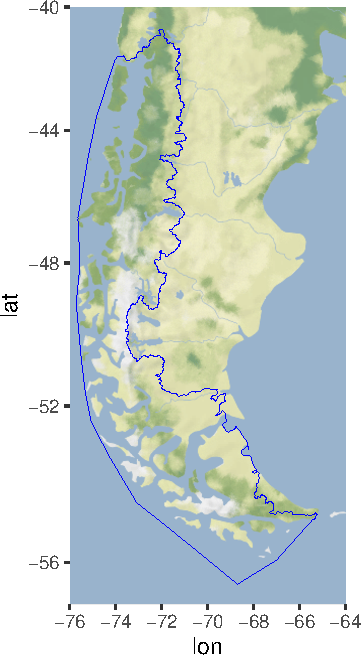
\includegraphics{Atlas_Ictiogeografico_files/figure-latex/studyareaplot-1} 

}

\caption{Area de estudio.}\label{fig:studyareaplot}
\end{figure}

El área de estudio resultante se aprecia en la Figura
\ref{fig:studyareaplot}.

\section{Conjuntos de datos
analizados}\label{conjuntos-de-datos-analizados}

Se incluyeron 12 conjuntos de datos en el análisis para generar el
\emph{Atlas Ictiogeográfico de la Patagonia}. Cada uno fue examinado,
corregido en casos de errores, complementado con variables aplicables al
nivel del conjunto de datos, y re-formateado para conformar al estándar
DwC. Las siguientes secciones documentan el manejo que recibió cada
conjunto de datos. Luego, en el capítulo \emph{Consolidación del Atlas
Ictiogeográfico}, se combinan todos los conjuntos de datos para
conformar una gran tabla maestra que entre otras mejoras, se procesó
para identificar ocurrencias duplicadas.

Durante la preparación de este documento algunos de los conjuntos de
datos que habían sido incorporados fueron ingresados por las agencias de
origen al Global Biodiversity Information Facility (GBIF). Por ejemplo,
este es el caso de \emph{Base de datos del MMA}. Aquí preservamos los
capítulos originales que describen estos conjuntos de datos para
entender mejor su origen y trazabilidad, pero ahora los datos se
importan directamente desde GBIF. {[}\textbf{HERE}, check if we actually
did this at the end.{]}

\subsection{Datos empíricos de los
autores}\label{datos-empuxedricos-de-los-autores}

\emph{Nombre del conjunto de datos}: Fish Database Correa-Boisjoly\\
\emph{Referencia}: Correa, Cristián, Maryse Boisjoly (2025) Base de
datos empírica de peces de Chile. Valdivia, Chile. \citep{Correa2025}\\
\emph{Archivo}: \texttt{FishDatabase\_Correa\_Boisjoly\_2025-11-27.csv}

Este conjunto de datos corresponde a nuestros propios datos empíricos de
registros de ocurrencias de peces dulceacuícolas, estuarinos y diádromos
en la Patagonia. Algunos de estos registros ya han sido publicados antes
pero hay muchos inéditos. Las ocurrencias han sido documentadas en el
marco de un número de proyectos de investigación y sus respectivos
permisos de pesca de investigación durante los últimos veinte años. En
general, el foco de los muestreos ha sido documentar biodiversidad de
peces nativos e introducidos, abarcando un amplio rango de técnicas de
muestreo, hábitats y tallas, pero también se hicieron muestreos
específicos.

Nuestros datos empíricos se encuentran almacenados en una base de datos
relacional en formato MSAcess. A partir de esta, creamos una consulta
(Querry) incluyendo todas las ocurrencias de peces y un conjunto de
atributos o campos relevantes que, como se describe a continuación,
fueron homologados al estándar DwC.

\subsubsection{Lectura de datos}\label{lectura-de-datos}

A partir de la base de datos se exportó una tabla simple
(\texttt{FishDatabase\_Correa\_Boisjoly\_2025-11-27.csv}) que se importa
y analiza a continuación:

\begin{Shaded}
\begin{Highlighting}[]
\NormalTok{FishDB\_CC }\OtherTok{\textless{}{-}} \FunctionTok{read.csv}\NormalTok{(}\StringTok{"./data\_sources/Correa\_Boisjoly\_Collection/FishDatabase\_Correa\_Boisjoly\_2025{-}11{-}27.csv"}\NormalTok{, }\AttributeTok{fileEncoding =} \StringTok{"UTF{-}8"}\NormalTok{, }\AttributeTok{colClasses =} \FunctionTok{c}\NormalTok{(}
                   \StringTok{"character"}\NormalTok{, }\CommentTok{\#Site.name"            }
                   \StringTok{"character"}\NormalTok{, }\CommentTok{\#Locality"             }
                   \StringTok{"character"}\NormalTok{, }\CommentTok{\#Site..waypoint.2014." }
                   \StringTok{"numeric"}\NormalTok{,   }\CommentTok{\#Lat\_effort"           }
                   \StringTok{"numeric"}\NormalTok{,   }\CommentTok{\#Lon\_effort"           }
                   \StringTok{"character"}\NormalTok{, }\CommentTok{\#SiteGear\_FieldID"     }
                   \StringTok{"numeric"}\NormalTok{,   }\CommentTok{\#Year"                 }
                   \StringTok{"character"}\NormalTok{, }\CommentTok{\#Date"                 }
                   \StringTok{"character"}\NormalTok{, }\CommentTok{\#Fishing.effort\_Id"    }
                   \StringTok{"character"}\NormalTok{, }\CommentTok{\#Technique"            }
                   \StringTok{"numeric"}\NormalTok{,   }\CommentTok{\#Fish\_Id"              }
                   \StringTok{"character"}\NormalTok{, }\CommentTok{\#Given.ID"             }
                   \StringTok{"character"}\NormalTok{, }\CommentTok{\#YYYY.MM.DD"           }
                   \StringTok{"character"}\NormalTok{, }\CommentTok{\#Species"              }
                   \StringTok{"numeric"}\NormalTok{,   }\CommentTok{\#N.Individuals"        }
                   \StringTok{"character"}\NormalTok{, }\CommentTok{\#Preserved."           }
                   \StringTok{"character"}\NormalTok{, }\CommentTok{\#Crew"                 }
                   \StringTok{"character"}\NormalTok{, }\CommentTok{\#bibliographicCitation"}
                   \StringTok{"character"}  \CommentTok{\#associatedReferences"}
\NormalTok{                  ) ) }


\NormalTok{FishDB\_CC}\SpecialCharTok{$}\StringTok{"YYYY.MM.DD"} \OtherTok{\textless{}{-}} \FunctionTok{as.Date}\NormalTok{(FishDB\_CC}\SpecialCharTok{$}\StringTok{"YYYY.MM.DD"}\NormalTok{, }\AttributeTok{format =} \StringTok{"\%Y{-}\%m{-}\%d"}\NormalTok{)}
\end{Highlighting}
\end{Shaded}

\subsubsection{Filtrado y agregación de
datos}\label{filtrado-y-agregaciuxf3n-de-datos}

En primer lugar, se filtró para retener solamente los peces de este
conjunto de datos.

\begin{Shaded}
\begin{Highlighting}[]
\NormalTok{FishDB\_CC }\OtherTok{\textless{}{-}}\NormalTok{ FishDB\_CC }\SpecialCharTok{\%\textgreater{}\%}
    \FunctionTok{filter}\NormalTok{(}\SpecialCharTok{!}\NormalTok{(Species }\SpecialCharTok{\%in\%}\NormalTok{ inverts), }\SpecialCharTok{!}\FunctionTok{is.na}\NormalTok{(Species))}
\CommentTok{\# where inverts is a vector of names to exclude, mostly}
\CommentTok{\# invertebrates.}
\end{Highlighting}
\end{Shaded}

La tabla de peces resultante presentó 11449 filas o registros y 19
columnas o atributos. Las filas representan ocurrencias de individuos o
conjuntos de individuos, por lo que para los efectos de este proyecto es
pertinente agregar los datos (combinar filas) para obtener presencia de
especies en sitios, fechas y protocolos de muestreos distintos.

Antes de agregar o combinar filas, se corrigieron algunas anomalías con
el conteo de individuos para obtener el número de individuos registrado.
En particular, cuando el campo \texttt{N.Individuals} estaba vacío se
asumió n = 1 porque ese campo sirve sobre todo para acomodar conjuntos
de peces indicando su número.

\begin{Shaded}
\begin{Highlighting}[]
\CommentTok{\# Assume is.na(N.individuals) correspond to n = 1.}
\NormalTok{FishDB\_CC}\SpecialCharTok{$}\NormalTok{N.Individuals[}\FunctionTok{is.na}\NormalTok{(FishDB\_CC}\SpecialCharTok{$}\NormalTok{N.Individuals)] }\OtherTok{\textless{}{-}} \DecValTok{1}

\CommentTok{\# Lots of still uncounted fish (e.g., photos of fish in}
\CommentTok{\# trays) were originally flagged as N.Individuals = 999,}
\CommentTok{\# and here that value was replaced by NA (all from Valdivia}
\CommentTok{\# though).}
\NormalTok{FishDB\_CC }\OtherTok{\textless{}{-}}\NormalTok{ FishDB\_CC }\SpecialCharTok{\%\textgreater{}\%}
    \FunctionTok{mutate}\NormalTok{(}\AttributeTok{N.Individuals =} \FunctionTok{ifelse}\NormalTok{((}\FunctionTok{match}\NormalTok{(N.Individuals, }\DecValTok{999}\NormalTok{,}
        \AttributeTok{nomatch =} \DecValTok{0}\NormalTok{) }\SpecialCharTok{==} \DecValTok{1}\NormalTok{), }\ConstantTok{NA}\NormalTok{, N.Individuals))}
\end{Highlighting}
\end{Shaded}

Función para agregar los datos:

\begin{Shaded}
\begin{Highlighting}[]
\NormalTok{FishDB\_CC\_aggregated }\OtherTok{\textless{}{-}}\NormalTok{ FishDB\_CC }\SpecialCharTok{\%\textgreater{}\%}
    \FunctionTok{group\_by}\NormalTok{(Locality, Lat\_effort, Lon\_effort, Year, YYYY.MM.DD,}
\NormalTok{        Species) }\SpecialCharTok{\%\textgreater{}\%}
    \FunctionTok{summarise}\NormalTok{(}\AttributeTok{Fish\_Id =} \FunctionTok{first}\NormalTok{(Fish\_Id), }\AttributeTok{n =} \FunctionTok{sum}\NormalTok{(N.Individuals),}
        \AttributeTok{Technique =} \FunctionTok{paste}\NormalTok{(}\FunctionTok{unique}\NormalTok{(Technique), }\AttributeTok{collapse =} \StringTok{", "}\NormalTok{),}
        \AttributeTok{Site.name =} \FunctionTok{paste}\NormalTok{(}\FunctionTok{unique}\NormalTok{(Site.name), }\AttributeTok{collapse =} \StringTok{", "}\NormalTok{),}
        \AttributeTok{Crew =} \FunctionTok{paste}\NormalTok{(}\FunctionTok{unique}\NormalTok{(Crew), }\AttributeTok{collapse =} \StringTok{", "}\NormalTok{), }\AttributeTok{bibliographicCitation =}\NormalTok{ \{}
\NormalTok{            vals }\OtherTok{\textless{}{-}} \FunctionTok{as.character}\NormalTok{(bibliographicCitation)}
\NormalTok{            vals }\OtherTok{\textless{}{-}} \FunctionTok{trimws}\NormalTok{(vals)}
\NormalTok{            vals }\OtherTok{\textless{}{-}}\NormalTok{ vals[}\SpecialCharTok{!}\FunctionTok{is.na}\NormalTok{(vals)]}
\NormalTok{            vals }\OtherTok{\textless{}{-}}\NormalTok{ vals[}\SpecialCharTok{!}\NormalTok{(vals }\SpecialCharTok{\%in\%} \FunctionTok{c}\NormalTok{(}\StringTok{""}\NormalTok{, }\StringTok{"NA"}\NormalTok{, }\StringTok{"\textless{}NA\textgreater{}"}\NormalTok{, }\StringTok{"na"}\NormalTok{))]}
            \ControlFlowTok{if}\NormalTok{ (}\FunctionTok{length}\NormalTok{(vals) }\SpecialCharTok{==} \DecValTok{0}\NormalTok{)}
                \StringTok{""} \ControlFlowTok{else}\NormalTok{ vals[}\DecValTok{1}\NormalTok{]}
\NormalTok{        \}, }\AttributeTok{associatedReferences =}\NormalTok{ \{}
\NormalTok{            vals }\OtherTok{\textless{}{-}} \FunctionTok{as.character}\NormalTok{(associatedReferences)}
\NormalTok{            vals }\OtherTok{\textless{}{-}}\NormalTok{ vals[}\SpecialCharTok{!}\FunctionTok{is.na}\NormalTok{(vals)]}
\NormalTok{            vals }\OtherTok{\textless{}{-}} \FunctionTok{trimws}\NormalTok{(vals)}
\NormalTok{            vals }\OtherTok{\textless{}{-}}\NormalTok{ vals[}\SpecialCharTok{!}\NormalTok{(vals }\SpecialCharTok{\%in\%} \FunctionTok{c}\NormalTok{(}\StringTok{""}\NormalTok{, }\StringTok{"NA"}\NormalTok{, }\StringTok{"\textless{}NA\textgreater{}"}\NormalTok{, }\StringTok{"na"}\NormalTok{))]}
            \ControlFlowTok{if}\NormalTok{ (}\FunctionTok{length}\NormalTok{(vals) }\SpecialCharTok{==} \DecValTok{0}\NormalTok{) \{}
                \StringTok{""}
\NormalTok{            \} }\ControlFlowTok{else}\NormalTok{ \{}
\NormalTok{                parts }\OtherTok{\textless{}{-}} \FunctionTok{unlist}\NormalTok{(}\FunctionTok{strsplit}\NormalTok{(vals, }\StringTok{"}\SpecialCharTok{\textbackslash{}\textbackslash{}}\StringTok{s*}\SpecialCharTok{\textbackslash{}\textbackslash{}}\StringTok{|}\SpecialCharTok{\textbackslash{}\textbackslash{}}\StringTok{s*|;}\SpecialCharTok{\textbackslash{}\textbackslash{}}\StringTok{s*"}\NormalTok{))}
\NormalTok{                parts }\OtherTok{\textless{}{-}} \FunctionTok{trimws}\NormalTok{(parts)}
\NormalTok{                parts }\OtherTok{\textless{}{-}}\NormalTok{ parts[}\SpecialCharTok{!}\NormalTok{(parts }\SpecialCharTok{\%in\%} \FunctionTok{c}\NormalTok{(}\StringTok{""}\NormalTok{, }\StringTok{"NA"}\NormalTok{, }\StringTok{"\textless{}NA\textgreater{}"}\NormalTok{,}
                  \StringTok{"na"}\NormalTok{))]}
\NormalTok{                parts }\OtherTok{\textless{}{-}} \FunctionTok{unique}\NormalTok{(parts)}
                \ControlFlowTok{if}\NormalTok{ (}\FunctionTok{length}\NormalTok{(parts) }\SpecialCharTok{==} \DecValTok{0}\NormalTok{)}
                  \StringTok{""} \ControlFlowTok{else} \FunctionTok{paste}\NormalTok{(parts, }\AttributeTok{collapse =} \StringTok{" | "}\NormalTok{)}
\NormalTok{            \}}
\NormalTok{        \}, }\AttributeTok{.groups =} \StringTok{"drop\_last"}\NormalTok{) }\SpecialCharTok{\%\textgreater{}\%}
    \FunctionTok{ungroup}\NormalTok{()}
\end{Highlighting}
\end{Shaded}

Hubo muchas ocasiones en las que varios esfuerzos de muestreo
practicados en un mismo lugar y fecha se agruparon en una sola fila por
especie detectada. En otras palabras, algunas filas representan una
ocurrencia obtenida mediante varios protocolos de muestreo. Por tanto,
para simplificar, en lo sucesivo hemos optado por omitir identificadores
tales como \texttt{Effort\_Id} y \texttt{Fish\_Id}.

\subsubsection{Filtrado área de
estudio}\label{filtrado-uxe1rea-de-estudio}

Se aplicó un filtro espacial para extraer las ocurrencias dentro del
área de estudio

La versión agregando ocurrencias por fecha, sitio, y especie se redujo
de 11449 a 750 filas u ocurrencias (Figura \ref{fig:CCdataplot}).

\begin{figure}

{\centering 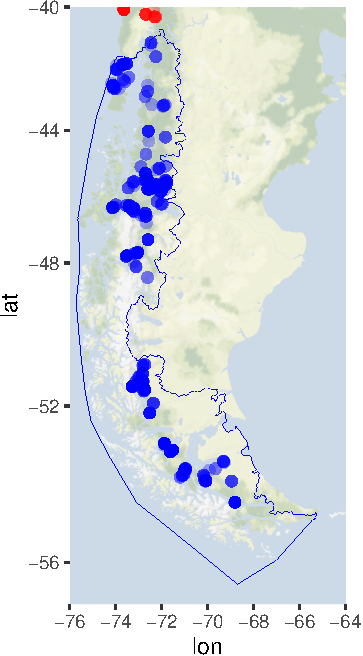
\includegraphics{Atlas_Ictiogeografico_files/figure-latex/CCdataplot-1} 

}

\caption{Distribución de ocurrencias de peces dulceacuícolas y diádromos  según los datos empíricos de los autores de este informe. Datos dentro del polígono del área de estudio en azul.}\label{fig:CCdataplot}
\end{figure}

Los peces reportados por este conjunto de datos dentro del área de
estudio se presentan en la Tabla \ref{tab:CCMBtaxa}.

\begingroup\fontsize{10}{12}\selectfont

\begin{longtable}[t]{>{\raggedright\arraybackslash}p{20em}>{\raggedright\arraybackslash}p{20em}}
\caption{\label{tab:CCMBtaxa}Lista de taxa encontrados en registros empíricos de Fish Database Correa-Boisjoly dentro del área de estudio.}\\
\toprule
Taxón & Taxón (continuación)\\
\midrule
Aplochiton marinus & Odontesthes brevianalis\\
Aplochiton sp. & Odontesthes hatcheri\\
Aplochiton taeniatus & Odontesthes regia\\
Aplochiton zebra & Odontesthes smitti\\
Brachygalaxias bulloki & Oncorhynchus kisutch\\
\addlinespace
Champsocephalus esox & Oncorhynchus masou\\
Cheirodon & Oncorhynchus mykiss\\
Cheirodon interruptus & Oncorhynchus tshawytscha\\
Cottoperca trigloides & Patagonotothen\\
Eleginops maclovinus & Patagonotothen sp\\
\addlinespace
Galaxias maculatus & Percichthys trucha\\
Galaxias maculatus & Salmo salar\\
Galaxias platei & Salmo trutta\\
Galaxias sp. & Salvelinus fontinalis\\
Geotria australis & Sardinops sagax\\
\addlinespace
Geotria macrostoma & Sebastes\\
Hatcheria macraei & \\
\bottomrule
\end{longtable}
\endgroup{}

\subsubsection{Homologación al formato
DwC}\label{homologaciuxf3n-al-formato-dwc}

Los campos más importantes fueron homologados como indica la siguiente
Tabla \ref{tab:CCMB_DwC}.

\begin{Shaded}
\begin{Highlighting}[]
\NormalTok{FishDB\_CC.Fields }\OtherTok{\textless{}{-}} \FunctionTok{colnames}\NormalTok{(FishDB\_CC\_aggregated)}

\NormalTok{DwC.eq }\OtherTok{\textless{}{-}}\NormalTok{ FishDB\_CC.Fields }\SpecialCharTok{\%\textgreater{}\%}
    \FunctionTok{recode}\NormalTok{(}\AttributeTok{Fish\_Id =} \StringTok{"occurrenceID"}\NormalTok{, }\AttributeTok{Site.name =} \StringTok{"locationRemarks"}\NormalTok{,}
        \AttributeTok{Locality =} \StringTok{"locality"}\NormalTok{, }\AttributeTok{Lat\_effort =} \StringTok{"decimalLatitude"}\NormalTok{,}
        \AttributeTok{Lon\_effort =} \StringTok{"decimalLongitude"}\NormalTok{, }\AttributeTok{Year =} \StringTok{"year"}\NormalTok{, }\AttributeTok{YYYY.MM.DD =} \StringTok{"eventDate"}\NormalTok{,}
        \AttributeTok{Species =} \StringTok{"scientificName"}\NormalTok{, }\AttributeTok{n =} \StringTok{"individualCount"}\NormalTok{, }\AttributeTok{Technique =} \StringTok{"samplingProtocol"}\NormalTok{,}
        \AttributeTok{Crew =} \StringTok{"recordedBy"}\NormalTok{, }\AttributeTok{bibliographicCitation =} \StringTok{"bibliographicCitation"}\NormalTok{,}
        \AttributeTok{associatedReferences =} \StringTok{"associatedReferences"}\NormalTok{)}

\FunctionTok{colnames}\NormalTok{(FishDB\_CC\_aggregated) }\OtherTok{\textless{}{-}}\NormalTok{ DwC.eq}
\NormalTok{FishDB\_CC.ready }\OtherTok{\textless{}{-}}\NormalTok{ FishDB\_CC\_aggregated[withinAE, ]}
\end{Highlighting}
\end{Shaded}

\begingroup\fontsize{7}{9}\selectfont

\begin{longtable}[t]{>{\raggedright\arraybackslash}p{20em}>{\raggedright\arraybackslash}p{20em}}
\caption{\label{tab:CCMB_DwC}Correspondencia entre atributos para homologar con DwC.}\\
\toprule
Fish Database Correa-Boisjoly & DwC equivalent\\
\midrule
Locality & locality\\
Lat\_effort & decimalLatitude\\
Lon\_effort & decimalLongitude\\
Year & year\\
YYYY.MM.DD & eventDate\\
\addlinespace
Species & scientificName\\
Fish\_Id & occurrenceID\\
n & individualCount\\
Technique & samplingProtocol\\
Site.name & locationRemarks\\
\addlinespace
Crew & recordedBy\\
bibliographicCitation & bibliographicCitation\\
associatedReferences & associatedReferences\\
\bottomrule
\end{longtable}
\endgroup{}

Además se añadieron algunos atributos del DwC que son constantes para
todo el conjunto de datos.

\begin{Shaded}
\begin{Highlighting}[]
\NormalTok{FishDB\_CC.ready}\SpecialCharTok{$}\NormalTok{license }\OtherTok{\textless{}{-}} \StringTok{"CC BY{-}NC 4.0"}
\NormalTok{FishDB\_CC.ready}\SpecialCharTok{$}\NormalTok{rightsHolder }\OtherTok{\textless{}{-}} \StringTok{"Cristian Correa, orcid.org/0000{-}0002{-}8608{-}6858"}
\NormalTok{FishDB\_CC.ready}\SpecialCharTok{$}\NormalTok{accessRights }\OtherTok{\textless{}{-}} \StringTok{"not{-}for{-}profit use only"}
\CommentTok{\# Add bibliographic citation where there is none (published}
\CommentTok{\# papers prevail when available).}
\NormalTok{FishDB\_CC.ready}\SpecialCharTok{$}\NormalTok{bibliographicCitation[}\FunctionTok{is.na}\NormalTok{(FishDB\_CC.ready}\SpecialCharTok{$}\NormalTok{bibliographicCitation) }\SpecialCharTok{|}
    \FunctionTok{trimws}\NormalTok{(FishDB\_CC.ready}\SpecialCharTok{$}\NormalTok{bibliographicCitation) }\SpecialCharTok{==} \StringTok{""}\NormalTok{] }\OtherTok{\textless{}{-}} \StringTok{"Correa, Cristian, and Maryse Boisjoly. 2025. Chilean fish collection and empirical database (Version 2025{-}11{-}27) [Unpublished dataset]."}
\NormalTok{FishDB\_CC.ready}\SpecialCharTok{$}\NormalTok{datasetName }\OtherTok{\textless{}{-}} \StringTok{"Correa{-}Boisjoly fish collection Version 2025{-}11{-}27"}
\NormalTok{FishDB\_CC.ready}\SpecialCharTok{$}\NormalTok{basisOfRecord }\OtherTok{\textless{}{-}} \StringTok{"Ocurrence"}
\end{Highlighting}
\end{Shaded}

La Tabla \ref{tab:CCMB_sample} muestra una muestra aleatoria de 10
registros.

\begin{Shaded}
\begin{Highlighting}[]
\NormalTok{tmp }\OtherTok{\textless{}{-}}\NormalTok{ FishDB\_CC.ready[}\FunctionTok{sample}\NormalTok{(}\FunctionTok{nrow}\NormalTok{(FishDB\_CC.ready), }\AttributeTok{size =} \DecValTok{10}\NormalTok{,}
    \AttributeTok{replace =}\NormalTok{ F), ]}

\NormalTok{tmp }\SpecialCharTok{\%\textgreater{}\%}
    \FunctionTok{kable}\NormalTok{(}\AttributeTok{longtable =}\NormalTok{ F, }\AttributeTok{landscape =} \ConstantTok{TRUE}\NormalTok{) }\SpecialCharTok{\%\textgreater{}\%}
    \FunctionTok{kable\_styling}\NormalTok{(}\AttributeTok{bootstrap\_options =} \FunctionTok{c}\NormalTok{(}\StringTok{"striped"}\NormalTok{, }\StringTok{"hover"}\NormalTok{, }\StringTok{"condensed"}\NormalTok{),}
        \AttributeTok{full\_width =}\NormalTok{ F, }\AttributeTok{latex\_options =} \FunctionTok{c}\NormalTok{(}\StringTok{"hold\_position"}\NormalTok{), }\AttributeTok{font\_size =} \DecValTok{5}\NormalTok{) }\SpecialCharTok{\%\textgreater{}\%}
    \FunctionTok{column\_spec}\NormalTok{(}\AttributeTok{column =} \DecValTok{1}\NormalTok{, }\AttributeTok{width =} \StringTok{"4em"}\NormalTok{) }\SpecialCharTok{\%\textgreater{}\%}
    \FunctionTok{column\_spec}\NormalTok{(}\AttributeTok{column =} \DecValTok{2}\NormalTok{, }\AttributeTok{width =} \StringTok{"4em"}\NormalTok{) }\SpecialCharTok{\%\textgreater{}\%}
    \FunctionTok{column\_spec}\NormalTok{(}\AttributeTok{column =} \DecValTok{3}\NormalTok{, }\AttributeTok{width =} \StringTok{"5em"}\NormalTok{) }\SpecialCharTok{\%\textgreater{}\%}
    \FunctionTok{column\_spec}\NormalTok{(}\AttributeTok{column =} \DecValTok{4}\NormalTok{, }\AttributeTok{width =} \StringTok{"5em"}\NormalTok{) }\SpecialCharTok{\%\textgreater{}\%}
    \FunctionTok{column\_spec}\NormalTok{(}\AttributeTok{column =} \DecValTok{5}\NormalTok{, }\AttributeTok{width =} \StringTok{"3em"}\NormalTok{) }\SpecialCharTok{\%\textgreater{}\%}
    \FunctionTok{column\_spec}\NormalTok{(}\AttributeTok{column =} \DecValTok{6}\NormalTok{, }\AttributeTok{width =} \StringTok{"5em"}\NormalTok{) }\SpecialCharTok{\%\textgreater{}\%}
    \FunctionTok{column\_spec}\NormalTok{(}\AttributeTok{column =} \DecValTok{7}\NormalTok{, }\AttributeTok{width =} \StringTok{"5em"}\NormalTok{) }\SpecialCharTok{\%\textgreater{}\%}
    \FunctionTok{column\_spec}\NormalTok{(}\AttributeTok{column =} \DecValTok{8}\NormalTok{, }\AttributeTok{width =} \StringTok{"2em"}\NormalTok{) }\SpecialCharTok{\%\textgreater{}\%}
    \FunctionTok{column\_spec}\NormalTok{(}\AttributeTok{column =} \DecValTok{9}\NormalTok{, }\AttributeTok{width =} \StringTok{"4em"}\NormalTok{) }\SpecialCharTok{\%\textgreater{}\%}
    \FunctionTok{column\_spec}\NormalTok{(}\AttributeTok{column =} \DecValTok{10}\NormalTok{, }\AttributeTok{width =} \StringTok{"2em"}\NormalTok{)  }\CommentTok{\#\%\textgreater{}\% }
\end{Highlighting}
\end{Shaded}

\begingroup\fontsize{5}{7}\selectfont

\begin{longtable}[t]{>{\raggedright\arraybackslash}p{4em}>{\raggedleft\arraybackslash}p{4em}>{\raggedleft\arraybackslash}p{5em}>{\raggedleft\arraybackslash}p{5em}>{\raggedright\arraybackslash}p{3em}>{\raggedright\arraybackslash}p{5em}>{\raggedleft\arraybackslash}p{5em}>{\raggedleft\arraybackslash}p{2em}>{\raggedright\arraybackslash}p{4em}>{\raggedright\arraybackslash}p{2em}llllllll}
\toprule
locality & decimalLatitude & decimalLongitude & year & eventDate & scientificName & occurrenceID & individualCount & samplingProtocol & locationRemarks & recordedBy & bibliographicCitation & associatedReferences & license & rightsHolder & accessRights & datasetName & basisOfRecord\\
\midrule
Lago Huelde, Río Cipresales & -42.58837 & -74.09985 & 2014 & 2014-02-25 & Salmo trutta & 4453 & 5 & Gill Net Experimental & Huelde & Cristian Correa, Maryse Boisjoly & Correa, Cristian, and Maryse Boisjoly. 2025. Chilean fish collection and empirical database (Version 2025-11-27) [Unpublished dataset]. &  & CC BY-NC 4.0 & Cristian Correa, orcid.org/0000-0002-8608-6858 & not-for-profit use only & Correa-Boisjoly fish collection Version 2025-11-27 & Ocurrence\\
Lago Castor & -45.60028 & -71.78156 & 2007 & 2007-02-08 & Oncorhynchus mykiss & 19 & 3 & Bottom gillnet S, Bottom gillnet L & Castor & Cristian Correa & Correa, C., Bravo, A.P., and Hendry, A.P. 2012. Reciprocal trophic niche shifts in native and invasive fish: salmonids and galaxiids in Patagonian lakes. Freshwater Biology 57(9): 1769–1781. & (Correa et al. 2012) \&\#124; (Correa and Hendry 2012) & CC BY-NC 4.0 & Cristian Correa, orcid.org/0000-0002-8608-6858 & not-for-profit use only & Correa-Boisjoly fish collection Version 2025-11-27 & Ocurrence\\
Lago Leon & -45.61615 & -71.84049 & 2009 & 2009-01-30 & Galaxias platei & 2166 & 3 & Bottom gillnet S & Leon & Cristian Correa & Correa, C., and Hendry, A.P. 2012. Invasive salmonids and lake order interact in the decline of puye grande Galaxias platei in western Patagonia lakes. Ecological Applications 22(3): 828–842. doi:10.1890/11-1174.1. & (Correa and Hendry 2012) & CC BY-NC 4.0 & Cristian Correa, orcid.org/0000-0002-8608-6858 & not-for-profit use only & Correa-Boisjoly fish collection Version 2025-11-27 & Ocurrence\\
Lago Toro & -45.52982 & -71.85324 & 2009 & 2009-10-30 & Galaxias platei & 3495 & 13 & Electric fishing & Toro & Cristian Correa & Correa, C., Bravo, A.P., and Hendry, A.P. 2012. Reciprocal trophic niche shifts in native and invasive fish: salmonids and galaxiids in Patagonian lakes. Freshwater Biology 57(9): 1769–1781. & (Correa et al. 2012) & CC BY-NC 4.0 & Cristian Correa, orcid.org/0000-0002-8608-6858 & not-for-profit use only & Correa-Boisjoly fish collection Version 2025-11-27 & Ocurrence\\
Río Simpson & -45.72747 & -72.08078 & 2007 & 2007-01-25 & Oncorhynchus tshawytscha & 1830 & 7 & Electric fishing & Simpson River & Cristian Correa & Correa, Cristian, and Maryse Boisjoly. 2025. Chilean fish collection and empirical database (Version 2025-11-27) [Unpublished dataset]. &  & CC BY-NC 4.0 & Cristian Correa, orcid.org/0000-0002-8608-6858 & not-for-profit use only & Correa-Boisjoly fish collection Version 2025-11-27 & Ocurrence\\
\addlinespace
Lago Aislado & -46.37539 & -73.24605 & 2014 & 2014-03-18 & Galaxias platei & 4545 & 2 & Hand Collected, Minnow Trap & Valle Exploradores & Cristian Correa, Maryse Boisjoly & Correa, Cristian, and Maryse Boisjoly. 2025. Chilean fish collection and empirical database (Version 2025-11-27) [Unpublished dataset]. &  & CC BY-NC 4.0 & Cristian Correa, orcid.org/0000-0002-8608-6858 & not-for-profit use only & Correa-Boisjoly fish collection Version 2025-11-27 & Ocurrence\\
Chaiten & -42.92081 & -72.71487 & 2007 & 2007-01-22 & Eleginops maclovinus & 3653 & 1 & Dip net & Chaiten & Cristian Correa & Correa, Cristian, and Maryse Boisjoly. 2025. Chilean fish collection and empirical database (Version 2025-11-27) [Unpublished dataset]. &  & CC BY-NC 4.0 & Cristian Correa, orcid.org/0000-0002-8608-6858 & not-for-profit use only & Correa-Boisjoly fish collection Version 2025-11-27 & Ocurrence\\
Estrecho de Magallanes & -53.68112 & -70.97443 & 2015 & 2015-02-20 & Galaxias maculatus & 6219 & 80 & Gill Net & Río Santa María & Fishermen & Correa, Cristian, and Maryse Boisjoly. 2025. Chilean fish collection and empirical database (Version 2025-11-27) [Unpublished dataset]. &  & CC BY-NC 4.0 & Cristian Correa, orcid.org/0000-0002-8608-6858 & not-for-profit use only & Correa-Boisjoly fish collection Version 2025-11-27 & Ocurrence\\
Río Caleta & -53.20692 & -71.61602 & 2015 & 2015-02-25 & Oncorhynchus kisutch & 5613 & 1 & Electric fishing & Río Caleta & Maryse Boisjoly, Jonathan Poblete & Correa, Cristian, and Maryse Boisjoly. 2025. Chilean fish collection and empirical database (Version 2025-11-27) [Unpublished dataset]. &  & CC BY-NC 4.0 & Cristian Correa, orcid.org/0000-0002-8608-6858 & not-for-profit use only & Correa-Boisjoly fish collection Version 2025-11-27 & Ocurrence\\
Río Ñireguao & -45.16493 & -72.10584 & 2014 & 2014-03-07 & Salmo trutta & 4515 & 1 & Gill Net Salmonera & Ñireguao River & Cristian Correa, Maryse Boisjoly & Correa, Cristian, and Maryse Boisjoly. 2025. Chilean fish collection and empirical database (Version 2025-11-27) [Unpublished dataset]. &  & CC BY-NC 4.0 & Cristian Correa, orcid.org/0000-0002-8608-6858 & not-for-profit use only & Correa-Boisjoly fish collection Version 2025-11-27 & Ocurrence\\
\bottomrule
\end{longtable}
\endgroup{}

\begin{Shaded}
\begin{Highlighting}[]
\CommentTok{\# column\_spec(column = 11, width = \textquotesingle{}6em\textquotesingle{}) \%\textgreater{}\%}
\CommentTok{\# column\_spec(column = 12, width = \textquotesingle{}3em\textquotesingle{}) \%\textgreater{}\%}
\CommentTok{\# column\_spec(column = 13, width = \textquotesingle{}4em\textquotesingle{})}
\end{Highlighting}
\end{Shaded}

\subsubsection{Respaldo}\label{respaldo}

\begin{Shaded}
\begin{Highlighting}[]
\FunctionTok{write.csv}\NormalTok{(FishDB\_CC.ready, }\StringTok{"./data\_sources/Correa\_Boisjoly\_Collection/Output\_FishDatabase\_Correa{-}Boisjoly.csv"}\NormalTok{,}
    \AttributeTok{fileEncoding =} \StringTok{"UTF{-}8"}\NormalTok{, }\AttributeTok{row.names =}\NormalTok{ F)}

\FunctionTok{saveRDS}\NormalTok{(FishDB\_CC.ready, }\StringTok{"./data\_sources/Correa\_Boisjoly\_Collection/Output\_FishDatabase\_Correa{-}Boisjoly.rds"}\NormalTok{)}
\end{Highlighting}
\end{Shaded}

\begin{Shaded}
\begin{Highlighting}[]
\NormalTok{knitr}\SpecialCharTok{::}\FunctionTok{knit\_exit}\NormalTok{()}
\end{Highlighting}
\end{Shaded}


\bibliography{bibliography/Biblio_Atlas_Ictio.bib}


\end{document}
